\chapter{運動量モードから局所量子場へ}

量子場とは何であり、それは粒子とどのように関係しているのか。基本的な数学的道具は調和振動子である。場は多くの可能な振動モードを含み、場を量子化することは、各モードに対して1つの量子調和振動子を組み合わせることに相当する。この構成は、まず有限な周期的空間で見るのが最も容易であり、そこでは許されるモードが離散的なリストをなす。

\section{周期的空間と許される波数}

1つの空間座標\(x\)をとり、距離\(L\)だけ離れた点を同一視する。この空間は周長\(L\)の円として思い描くことができる。これは有用な有限体積の技巧である。端点をもつ有限区間では、進行波は端で反射する。周期的区間では、波は反射せずにどちらの方向へも進み続けることができる。並進対称性、したがって運動量保存則は保たれつつ、無限体積の複雑さは一時的に取り除かれる。

平面波は
\begin{equation}
e^{ikx}.
\end{equation}
の形をとる。円を一周した後、波は元の値に戻らなければならない。波は\(x=0\)で\(1\)に等しいので、周期性は
\begin{equation}
e^{ikL}=1.
\end{equation}
を要求する。なぜ\(2\pi\)の整数倍がこの条件を満たすのか。オイラーの公式により
\begin{align}
e^{i2\pi n}
&=\cos(2\pi n)+i\sin(2\pi n)\\
&=1,
\qquad n\in\mathbb Z.
\end{align}
となる。任意の整数回の周期の後、余弦は\(1\)であり、正弦は\(0\)である。したがって、
\begin{equation}
kL=2\pi n,
\qquad
k=\frac{2\pi n}{L},
\qquad n\in\mathbb Z.
\end{equation}
となる。量\(k\)は波数である。整数\(n\)は許される波数にラベルを付けるものであり、まだ粒子を数えているわけではない。

同じ条件は波長を用いて表すこともできる。波長とは位相が1周期だけ進む距離であるから、
\begin{equation}
k\lambda=2\pi,
\qquad
k=\frac{2\pi}{\lambda}.
\end{equation}
となる。長い波長は小さな波数を、短い波長は大きな波数をもつ。周期性の条件は、円の周りに整数個の波長が収まることを述べている。

量子力学的な波に対して、運動量は
\begin{equation}
p=\frac{h}{\lambda}
=\frac{2\pi\hbar}{\lambda}
=\hbar k.
\end{equation}
である。したがって、\(k\)と\(p\)は因子\(\hbar\)だけ異なる。正と負の\(k\)は、反対方向に進む波と、反対向きの運動量をもつ粒子を表す。\(\hbar=1\)とする単位系では、\(k\)をそれ以上区別せずに運動量と呼ぶのが通例である。

許される各\(k\)に対して、そのモードには何個かの量子が存在しうる。これにより第二の整数が導入される：
\begin{equation}
n(k)=\text{number of quanta with wave number }k.
\end{equation}
これは占有数と呼ばれる。\(k=2\pi n/L\)における整数はモードを指定し、\(n(k)\)はそのモードを占める粒子の数を示す。占有数は正負いずれの\(k\)についても与えなければならない。

\begin{classroomqa}
\lecturetimestamp{00:11:58}
\audiencequestion{\(k\)自体は整数か。}
\lecturerresponse{いいえ。波数は\(2\pi/L\)の整数倍である：\(k=2\pi n/L\)。この式の整数\(n\)は許される運動量にラベルを付けるものであり、モード内の量子を数える占有数\(n(k)\)とは別のものである。}
\end{classroomqa}

\section{占有数状態とモード演算子}

量子状態はベクトル、すなわち線形要素である。状態ベクトルは加算したり数で乗じたりすることができ、演算子はそれらに作用して別の状態ベクトルを生み出す。観測可能な実量はエルミート演算子で表される。これらの初歩的な事実は、多粒子状態と場の両方が線形結合と演算子から構成されるため、ここで重要となる。

次のようにおく：
\begin{equation}
k_j=\frac{2\pi j}{L},
\qquad j\in\mathbb Z.
\end{equation}
多粒子状態の便利なラベルは、占有数の列全体である。表示された成分に対して略記\(n_j\equiv n(k_j)\)を用いて、
\begin{equation}
\big|\{n(k_j)\}\big\rangle
=
\big|\ldots,n_{-2},n_{-1},n_0,n_1,n_2,\ldots\big\rangle.
\end{equation}
と書く。成分\(n(k_1)\)は第1の正運動量モードの粒子数であり、\(n(k_2)\)は第2のモードの粒子数であり、以下同様である。この列は両方向に無限に続く。

\begin{figure}[t]
\centering
\includegraphics[width=0.72\textwidth]{lecture_03_figure_02.png}
\caption{許される運動量モードに対する占有数\(n(k)\)。}
\lectureframe{00:15:04}
\end{figure}

各運動量モードは調和振動子である。したがって、それは生成演算子と消滅演算子をもつ。最初に\(a^{+}(k)\)および\(a^{-}(k)\)と書かれた記法は、\(a^\dagger(k)\)および\(a(k)\)と書かれることになる。それらの作用は
\begin{align}
a^\dagger(k)\big|\ldots,n(k),\ldots\big\rangle
&=
\sqrt{n(k)+1}\notag\\
&\quad{}\times
\big|\ldots,n(k)+1,\ldots\big\rangle,
\\
a(k)\big|\ldots,n(k),\ldots\big\rangle
&=
\sqrt{n(k)}\,
\big|\ldots,n(k)-1,\ldots\big\rangle.
\end{align}
である。演算子\(a^\dagger(k)\)は\(k\)に対応するスロットに作用し、その占有数を1つ増やし、状態に\(\sqrt{n(k)+1}\)を掛ける。演算子\(a(k)\)は同じスロットの占有数を減らし、\(\sqrt{n(k)}\)を与える。許される運動量ごとに、このような対が1つ存在する。

\begin{figure}[t]
\centering
\includegraphics[width=0.58\textwidth]{lecture_03_figure_03.png}
\caption{運動量モード\(k\)に付随する生成演算子と消滅演算子。}
\lectureframe{00:17:14}
\end{figure}

\section{フーリエ係数が演算子になる}

これらの振動子演算子と場との結びつきは、通常の古典的フーリエ級数から始まる。周期的区間上の複素古典場は
\begin{align}
\psi(x)&=\sum_k \alpha(k)e^{ikx},\\
\psi^*(x)&=\sum_k \alpha^*(k)e^{-ikx},
\end{align}
と書ける。ここで各和は許される値\(k=2\pi n/L\)にわたる。これは場をサインとコサインで展開することと等価である。

複素場は実部と虚部をもつ。その複素共役は虚部の符号を反転させ、\(e^{ikx}\)は\(e^{-ikx}\)となる。すべての係数\(\alpha(k)\)を指定すれば古典場が指定される。\(\alpha(k)\)がわかれば\(\alpha^*(k)\)を独立に指定する必要はないが、各係数の実部と虚部は別々の実量である。それらは対応するフーリエ成分の振幅として測定できる。この意味で、複素係数は二つの古典的可観測量をまとめたものである。

量子化はこれらの古典的フーリエ係数を演算子に置き換える。通常の等号は異なる種類の対象を同一視してしまうので、置き換え規則として書く方がよい：
\begin{equation}
\alpha(k)\rightsquigarrow a(k),
\qquad
\alpha^*(k)\rightsquigarrow a^\dagger(k).
\end{equation}
フーリエの符号の選び方を一貫させると、量子場は
\begin{align}
\Psi(x)&=\sum_k a(k)e^{ikx},\\
\Psi^\dagger(x)&=\sum_k a^\dagger(k)e^{-ikx}.
\end{align}
\editorialnote{口頭の議論はフーリエ符号の規約を変更し、後にそれを問い直す。ここで用いられる共役対は、より明確な場の展開と位置状態の計算に見られる規約である：\(\Psi\)は\(e^{ikx}\)を伴い、\(\Psi^\dagger\)は\(e^{-ikx}\)を伴う。すべての符号を一貫して反転しても同じ構成を記述することになる。}

今のところ、これは定義である：量子場とは係数が演算子であるフーリエ和である。より完全な正当化には、これらの演算子が適切な極限で古典的係数を再現することを示す必要があり、そのためには何らかの力学が必要である。その問いは後回しにされる。すでに明らかなのは、場自体が演算子であり、そのフーリエ係数の間の関係が調和振動子の生成・消滅関係であるということである。

\begin{classroomqa}
\lecturetimestamp{00:26:48}
\audiencequestion{生成演算子と消滅演算子を導入することは、力学が必然的に粒子を生成・消滅させることを意味するのか？}
\lecturerresponse{いいえ。これらの演算子は占有数を変える数学的操作である。自然の法則が実際に粒子数を変えるかどうかは力学に関する問いである。力学がそのような変化を許すならば、これらの演算子はそれを記述するための自然な言語を提供する。}
\end{classroomqa}

\section{散乱と粒子数の変化}

まず粒子数を変えない過程を考える。最初に存在する唯一の粒子が運動量\(k_7\)をもつとしよう。占有数表記では、その状態は七番目のスロットに\(1\)をもち、他はすべてゼロである：
\begin{equation}
|k_7\rangle
=
|\ldots,0,\underset{k_7}{1},0,\ldots\rangle.
\end{equation}
散乱過程はその運動量を\(k_7\)から\(k_9\)へ変える。まさにこの変化を引き起こす演算子は
\begin{equation}
a^\dagger(k_9)a(k_7).
\end{equation}
である。右端の演算子が最初に作用する：それは\(k_7\)スロットの粒子を除去する。次に左の演算子が\(k_9\)スロットに粒子を生成する。

\begin{classroomqa}
\lecturetimestamp{00:31:37}
\audiencequestion{この\(k_7\to k_9\)過程では平方根の因子はどこから入るのか？}
\lecturerresponse{消滅因子は\(\sqrt{n(k_7)}=\sqrt{1}=1\)である。その除去の後、系は全ゼロ状態にある。\(k_9\)モードは空なので、生成因子は\(\sqrt{n(k_9)+1}=\sqrt{1}=1\)である。したがって、この一粒子の例ではどちらの因子も数値係数を変えない。}
\end{classroomqa}

両方のステップを実行しよう。消滅は
\begin{align}
a(k_7)|k_7\rangle
&=
\sqrt{1}\,|\ldots,0,0,0,\ldots\rangle\\
&=|0\rangle.
\end{align}
を与える。全ゼロ状態は真空である。それは粒子のない状態であり、この単純な振動子の集まりでは基底状態でもある。次に空の\(k_9\)モードへの生成は
\begin{equation}
a^\dagger(k_9)|0\rangle
=\sqrt{0+1}\,|k_9\rangle
=|k_9\rangle.
\end{equation}
を与える。したがって、
\begin{equation}
a^\dagger(k_9)a(k_7)|k_7\rangle=|k_9\rangle.
\end{equation}
スロットごとに見れば、唯一の\(1\)は七番目の運動量モードから九番目へ移っただけである。占有数が一度も一を超えなかったので、両方の平方根因子は一に等しかった。すでに占有されたモードが関与するやいなや、それらは重要になる。

この一対一の過程は通常の一粒子量子力学でも記述できよう：一つの粒子がその運動量を変える。占有数表記が不可欠になるのは、粒子数が変化しうる場合である。例えば、
\begin{equation}
a^\dagger(k_9)a^\dagger(k_{16})a(k_7)|k_7\rangle
=|k_9,k_{16}\rangle
\end{equation}
は、モード\(k_7\)の一つの入射粒子から、\(k_9\)に一つと\(k_{16}\)に一つという二つの出射粒子への数学的変化を記述する。標的は入射粒子を吸収し、二つの出射粒子を放出し、必要などんな反跳でも引き受けてよい。そのような過程は一粒子に制限されたヒルベルト空間では表現できないが、占有数が変わりうる状態空間には自然に収まる。演算子の表式それ自体は自然の法則ではない；それは数を変える法則を書き表すための言語である。

\section{一点における場の演算子}

位置空間の演算子\(\Psi^\dagger(x)\)は何を生成するか。量子状態は線形空間をなす。すなわち、運動量状態に複素係数を掛けて加え合わせることで新たな状態を作ることができる。真空から始めよう。すべてのモードが空であるから、
\begin{equation}
\Psi(x)|0\rangle=0.
\end{equation}
右辺のゼロはゼロベクトルである。消滅演算子は取り除くべき粒子を見つけることができない。

共役場は異なる働きをする。
\begin{align}
\Psi^\dagger(x)|0\rangle
&=\sum_k e^{-ikx}a^\dagger(k)|0\rangle\\
&=\sum_k e^{-ikx}|k\rangle,
\end{align}
ここで
\begin{equation}
|k\rangle=a^\dagger(k)|0\rangle
\end{equation}
は運動量\(\hbar k\)の一粒子状態である。

\begin{figure}[t]
\centering
\includegraphics[width=0.70\textwidth]{lecture_03_figure_05.png}
\caption{形式的位置空間状態\(\Psi^\dagger(x)|0\rangle\)を一粒子運動量状態で展開したもの。}
\lectureframe{00:43:16}
\end{figure}

形式的に、また規格化を除いて、この和は一粒子量子力学の一般化された位置状態である。\footnote{運動量モードが無限に多く存在する場合、厳密に局在した位置状態は規格化不可能である。有限の運動量カットオフを課し、その代わりに打ち切られた和を規格化すれば、\(x\)を中心とする鋭く局在した波束が得られる。}運動量固有状態に係数\(e^{-ikx}\)を組み合わせると、\(x\)における局在が生じる。この形式的な意味で、
\begin{equation}
\Psi^\dagger(x)\ \text{creates a particle at position }x,
\end{equation}
一方
\begin{equation}
\Psi(x)\ \text{annihilates a particle at position }x.
\end{equation}
モード演算子\(a^\dagger(k)\)は確定した運動量をもつ粒子を生成する。場の演算子\(\Psi^\dagger(x)\)は、形式的に\(x\)に局在する、許された運動量状態のコヒーレントな重ね合わせを生成する。

形式的で規格化されていない和においては、すべての係数\(e^{-ikx}\)の大きさは1である。有限のカットオフがある場合、規格化された打ち切られた状態は、保持された運動量に対して等しい大きさの係数をもち、その位相が\(x\)の近くに鋭く局在した波束を生み出す。これが量子場と粒子の間の初等的な関係である。

今は特殊相対論的な複雑さを無視すれば、この模型において\(\Psi^\dagger(x)\)は\(x\)に粒子を生成する。相対論的な場には改良が必要であるが、演算子値のフーリエ展開と、運動量モードの演算子と位置空間の演算子の区別は基本的なものであり続ける。

\begin{classroomqa}
\lecturetimestamp{00:44:59}
\audiencequestion{\(x\)は周期的な円周上の一点なのか、そして円周が大きくなると何が起こるのか。}
\lecturerresponse{はい。有限の模型では、\(x\)は円周上の点である。隣り合う許された波数は\(2\pi/L\)だけ離れている。\(L\)が大きくなると、その間隔は小さくなるので、望むどの運動量に対しても、それにいくらでも近い許された値が存在する。無限体積の極限では、\(k\)にわたる和は\(k\)にわたる積分に置き換えられる。まず離散的な和を理解することが有用である。}
\end{classroomqa}

\section{局所的な粒子反応}

\(\Psi(x)\)と\(\Psi^\dagger(x)\)が一点において粒子を消滅させ生成すると解釈されたならば、局所性を直接表現することができる。\(x\)に鋭く局在した標的に粒子が吸収され、一方、出ていく粒子が一つはアルファ・ケンタウリの近くに、もう一つはベテルギウスの近くに突然現れると想像しよう。そのような反応は非局所的である。その離れた事象は通常の伝播によって結びつけることができない。

まず要求を弱めて、出ていく粒子が標的の周りの小さな領域内のどこかで放出されることを許すこともできる。正確な局所的理想化はより強い。すなわち、入射粒子が\(x\)で吸収されるならば、出ていく粒子はその同じ点で生成される。代わりに離れた点で評価された場を用いれば、非局所的な演算子積を記述することになる。したがって局所的な1対2の操作は
\begin{equation}
\Psi^\dagger(x)\Psi^\dagger(x)\Psi(x).
\end{equation}
最も右の場は\(x\)で入射粒子を取り除き、その左の二つの場はそこで二つの出ていく粒子を生成する。\footnote{局所的な1対2の模式図は00で述べられた反応に対応する。47:38--00:49:13。}

\begin{figure}[t]
\centering
\begin{tikzpicture}[scale=1.0]
\draw[->] (-2.2,0) -- (0,0);
\fill (0,0) circle (2.2pt);
\draw[->] (0,0) -- (2.0,1.1);
\draw[->] (0,0) -- (2.0,-1.1);
\node at (-1.25,0.3) {$k_{\mathrm{initial}}$};
\node[right] at (0.05,0.05) {$x$};
\node at (1.48,1.34) {$\ell$};
\node at (1.48,-1.34) {$m$};
\end{tikzpicture}
\caption{一つの入射粒子が\(x\)で吸収され、二つの出ていく粒子が同じ点で生成される。}
\end{figure}

入射状態が確定した波数\(k_{\mathrm{initial}}\)の一粒子を含むとしよう。出ていく運動量を決定するには、局所的な場の運動量空間展開を代入する。固定された運動量ラベルとダミーの和の添字を区別することが重要である。
\begin{align}
\Psi(x)&=\sum_q a(q)e^{iqx},\\
\Psi^\dagger(x)&=\sum_\ell a^\dagger(\ell)e^{-i\ell x}.
\end{align}
と書く。添字\(q\)は和をとられるが、\(k_{\mathrm{initial}}\)は特定の占有された入射モードを表す。\(\Psi^\dagger(x)\)の二つのコピーにも独立なダミー添字、たとえば\(\ell\)と\(m\)が必要である。一つの添字を再利用すると、二つの独立な和を誤って結びつけてしまう。ここで\(\ell\)と\(m\)は波数であり、\(m\)は質量を表すのではない。

具体的な描像は、\(x\) に局在する原子に光子が衝突し、その後その点から2個の光子が放出されるというものである。ここで用いた単純な場は、完全に相対論的な光子場よりも非相対論的粒子に適しているため、光子という言葉は演算子の帳簿付けを例示しているにすぎない。

まず消滅場が作用する：
\begin{align}
\Psi(x)|k_{\mathrm{initial}}\rangle
&=\sum_q e^{iqx}a(q)a^\dagger(k_{\mathrm{initial}})|0\rangle.
\end{align}
\(q=k_{\mathrm{initial}}\) をもつ項以外のすべての項は消える。消滅演算子は自身のモードにある粒子を見つけなければならない。したがって
\begin{equation}
\Psi(x)|k_{\mathrm{initial}}\rangle
=e^{ik_{\mathrm{initial}}x}|0\rangle.
\end{equation}
次に2つの生成場により
\begin{align}
&\Psi^\dagger(x)\Psi^\dagger(x)\Psi(x)
|k_{\mathrm{initial}}\rangle
\\
&\quad=
e^{ik_{\mathrm{initial}}x}
\sum_{\ell,m}
e^{-i\ell x}e^{-imx}
a^\dagger(\ell)a^\dagger(m)|0\rangle
\\
&\quad=
\sum_{\ell,m}
e^{i(k_{\mathrm{initial}}-\ell-m)x}
a^\dagger(\ell)a^\dagger(m)|0\rangle.
\end{align}
\(\ell\) と \(m\) が等しくない場合、演算子状態は \(|\ell,m\rangle\) と表してよい：2つのモードのそれぞれに1個の粒子が占有している。最終結果は、そのような2粒子運動量配置すべてにわたる和であり、位相は入射運動量と出射運動量によって決まる。

\begin{classroomqa}
\lecturetimestamp{01:00:36}
\audiencequestion{2つの生成演算子は可換か？}
\lecturerresponse{はい。すべての生成演算子は互いに可換であり、すべての消滅演算子も互いに可換である。生成演算子と消滅演算子は、異なるモードを参照するときには可換である；同じモードに対してはそれらの交換子は非零である。}
\end{classroomqa}

\begin{classroomqa}
\lecturetimestamp{01:01:34}
\audiencequestion{2つの出射運動量は運動量保存を満たすべきか？}
\lecturerresponse{表示された粒子だけでは運動量を保存する必要はない。原子または標的が反跳しうるからである。差 \(k_{\mathrm{initial}}-\ell-m\) は標的に移された運動量である。標的を含めた全運動量が保存量である。}
\end{classroomqa}

係数 \(e^{i(k_{\mathrm{initial}}-\ell-m)x}\) は純粋な位相であるから、その大きさは1である。一見すると、これはすべての対 \((\ell,m)\) に対して等しい確率重みを示唆する。しかしながら、2つのラベルが一致する場合には重要な但し書きがある。

\(\ell=m\) ならば、最初の生成演算子はモード \(m\) に1個の粒子を入れ、2番目はすでに1回占有されたモードに作用する：
\begin{align}
a^\dagger(m)a^\dagger(m)|0\rangle
&=a^\dagger(m)|1_m\rangle\\
&=\sqrt{2}\,|2_m\rangle.
\end{align}
したがって、1つのモードにおける二重生成には余分な振幅 \(\sqrt{2}\) が伴う。振幅を2乗すると、確率に因子 \(2\) が生じる。

\begin{classroomqa}
\lecturetimestamp{01:04:54}
\audiencequestion{生成係数が \(n+1\) を含むからといって、\(\ell\) と \(m\) は1だけ異ならなければならないのか？}
\lecturerresponse{いいえ。記号 \(\ell\) と \(m\) は運動量モードをラベルする。\(\sqrt{n+1}\) における \(n\) は、生成演算子が作用する特定のモードの占有数である。運動量ラベルと粒子数は別個の整数である。}
\end{classroomqa}

\begin{figure}[t]
\centering
\includegraphics[width=0.92\textwidth]{lecture_03_figure_06.png}
\caption{局所的な1→2粒子振幅の運動量空間展開。}
\lectureframe{01:05:44}
\end{figure}

この構成における粒子は同一である。したがって \(\sqrt{2}\) はボソン的占有因子であり、第1の粒子と第2の粒子を区別するラベルではない。これを2乗すると、暫定的には、同一運動量の結果が1つの等しくない運動量の項よりも2倍確からしくなるように見える。この比較は、二重和の項を注意深く数えたうえで再検討する必要がある。

\begin{classroomqa}
\lecturetimestamp{01:06:43}
\audiencequestion{複雑な反応では、生成演算子と消滅演算子の順序はどのように選ばれるのか？}
\lecturerresponse{すべての生成演算子を左に、消滅演算子を右に置いた式は正規順序と呼ばれる。その形では、最も右の演算子がまず入射粒子を取り除き、残りの演算子が出射粒子を生成する。}
\end{classroomqa}

混合した生成--消滅の対を並べ替えることは、一般には単純な置換ではない：交換子を用いなければならず、同じモードに対してはこれが追加の項を生じる。\footnote{この交換子に関する但し書きは、01 における非形式的な正規順序の議論に対する編集上の訂正である：06：43。}

\begin{classroomqa}
\lecturetimestamp{01:07:30}
\audiencequestion{運動量振幅がすべて同じ大きさをもつならば、``2倍確からしい'' といった言明は何を意味するのか？}
\lecturerresponse{有限の空洞を念頭に置きなさい。その許される運動量は離散的であるから、確率はモードごとに比較できる。この比較は連続体中の孤立した点の確率の間の比較ではない。}
\end{classroomqa}

\(\ell\ne m\) に対して、制限のない二重和は両方の順序の項を含む
\begin{equation}
a^\dagger(\ell)a^\dagger(m)|0\rangle
\quad\text{and}\quad
a^\dagger(m)a^\dagger(\ell)|0\rangle.
\end{equation}

\begin{classroomqa}
\lecturetimestamp{01:08:24}
\audiencequestion{\(\ell\ne m\) のとき、同じ最終状態が二重和の中に2回、1回は \((\ell,m)\) として、もう1回は \((m,\ell)\) として現れるのか？}
\lecturerresponse{はい。\(\ell\ne m\) ならば、項 \((\ell,m)\) と \((m,\ell)\) の両方が現れ、生成演算子が可換であるため、それらは同じ物理的状態を記述する。}
\end{classroomqa}

順序付けられた2つの項は等しいので、定量的なチャネル比較を行う前に、状態の規格化とこの二重計数を処理しなければならない。信頼できる代数的結論はより狭く、以下の議論には十分である：すでに\(n\)個の同一のボソンが占有しているモードに生成すると、因子\(\sqrt{n+1}\)が生じる。

\section{自発放出と誘導放出}

より明快な例が平方根因子を分離する。\(x\)に局在する物体が1個の光子を放出するとしよう。光子場が真空から始まるなら、出ていく状態は
\begin{align}
\Psi^\dagger(x)|0\rangle
&=\sum_k e^{-ikx}a^\dagger(k)|0\rangle\\
&=\sum_k e^{-ikx}|k\rangle.
\end{align}
である。この単純化された模型では、すべての運動量は等しい振幅の大きさをもつ。すでに光子が存在しないので、放出は自発的である。

次に、モード\(\ell\)にすでに1個の光子があるとしよう。同じ局所生成場を作用させると、2種類の項が得られる：
\begin{equation}
\Psi^\dagger(x)|\ell\rangle
=
\sum_{k\ne\ell}e^{-ikx}|k,\ell\rangle
+e^{-i\ell x}\sqrt{2}\,|2_\ell\rangle.
\end{equation}
\(k\ne\ell\)に対しては、演算子は空のモードに生成するので、係数は\(\sqrt{0+1}=1\)である。\(k=\ell\)に対しては、占有されたモードに生成するので、係数は\(\sqrt{1+1}=\sqrt{2}\)である。元の光子は傍観者であり、新しい光子はその占有されたモードへ優先的に放出される。

\begin{classroomqa}
\lecturetimestamp{01:16:14}
\audiencequestion{誘導放出を引き起こすには、既存の光子が同じ位置になければならないのか。}
\lecturerresponse{この単純化された計算は、同じ運動量モードの占有を指しており、2つの粒子が1つの鋭く定義された位置にあることを指しているのではない。粒子は正確な位置と正確な運動量を同時にもつことはできない。実在の光子は波束で記述され、一方、空洞の理想化は確定した離散モードを与える。その設定では、増強はすでに占有された空洞モードへのものである。}
\end{classroomqa}

モード\(\ell\)が最初に\(n_\ell\)個の光子を含むなら、
\begin{equation}
a^\dagger(\ell)
|\ldots,n_\ell,\ldots\rangle
=
\sqrt{n_\ell+1}
\,|\ldots,n_\ell+1,\ldots\rangle.
\end{equation}
である。したがって確率は因子\(n_\ell+1\)だけ増強される。すでに1個の光子が存在する場合、因子は\(2\)である。モードに100個の光子がある場合、振幅因子は\(\sqrt{101}\)であり、そのモードへの放出確率は空モードの値の\(101\)倍である。ボソンモードにすでに存在する量子が多ければ多いほど、次の量子はそのモードへ放出されやすくなる。これが誘導放出である。

同じ占有効果は散乱反応にも現れる。衝突がある粒子をいくつかのモードに生成しうるなら、既存の占有は占有されたモードへの生成を増強する。これはこの振動子代数の一般的性質であり、原子崩壊に特有の奇妙さではない。

\begin{classroomqa}
\lecturetimestamp{01:18:15}
\audiencequestion{先ほどの2粒子過程で、新たに生成された2つの粒子の運動量が異なる場合でも、それらは依然としてより大きな重みをもつのか。}
\lecturerresponse{はい。順序付けられた二重和では、運動量が等しくない対は2つの順序で現れる。同一モード因子\(\sqrt{2}\)はその組合せ上の差を減らすが、それ自体では消し去らない。}
\end{classroomqa}

以前と同様、物理的なチャネル比較には依然として一貫した状態の規格化と計数が必要である。

\begin{classroomqa}
\lecturetimestamp{01:18:30}
\audiencequestion{それは、ボソンがすでに占有された運動量状態へ引き寄せられることを意味するのか。}
\lecturerresponse{いいえ。文字通りの力や引力は存在しない。この増強は、粒子の同一性とボソン生成演算子における平方根因子の統計的帰結である。}
\end{classroomqa}

2つの名称を区別しておくと有用である。光子が存在しない場合、係数は\(n=0\)で始まり、自発放出に対応する単位因子を与える。光子がすでに存在する場合、因子\(n+1\)がそれらのモードへの放出をより起こりやすくする。これが誘導放出である。

古典的な類似がある。既存の電磁波が原子を通り過ぎると、その電子を駆動する。駆動された電子は、波がなければそうであるよりも強く放射し、付加された放射は駆動波の方向と波数に従う。量子論的な言明では、既存の波は占有された光子モードに置き換えられる：既存の量子が同じモードにより多くの量子の生成を誘導する。

この調和振動子代数に従う粒子はボソンである。それらは占有された状態に蓄積する統計的傾向をもつが、互いにそれらの状態へ引き寄せ合うことはない。粒子はボソンとフェルミオンという2つの統計的種類に分かれる。現在の構成はボソン的であり、反対のフェルミオン的振る舞いは後で扱う。

\section{ボソン代数と粒子密度}

すべての運動量モードに対して生成演算子と消滅演算子が存在する。それらの代数は
\begin{align}
[a^\dagger(k),a^\dagger(\ell)]&=0,\\
[a(k),a(\ell)]&=0,\\
[a(k),a^\dagger(\ell)]&=\delta_{k\ell}.
\end{align}
である。ここで
\begin{equation}
[A,B]=AB-BA,
\end{equation}
であり、クロネッカーのデルタは
\begin{equation}
\delta_{k\ell}=
\begin{cases}
1,&k=\ell,\\
0,&k\ne\ell.
\end{cases}
\end{equation}
である。生成演算子は運動量が等しくても異なっても互いに可換であり、消滅演算子も同様である。混合対は異なる運動量に対して可換であり、同じ運動量に対してはおなじみの単一振動子の交換関係をもつ。

\(\Psi(x)\)のフーリエ定義とともに、これらの関係は最も単純なボソン量子場を定義する。この場の役割は、モードごとに、あるいは指定された位置において、粒子を生成および消滅させることである。

ここで演算子
\begin{equation}
\int_0^L dx\,\Psi^\dagger(x)\Psi(x).
\end{equation}
を考えよう。あらかじめ名前を付けるのではなく、実際に計算してみる。フーリエ展開を代入すると
\begin{align}
\int_0^L dx\,\Psi^\dagger(x)\Psi(x)
&=
\sum_{k,\ell}a^\dagger(k)a(\ell)
\int_0^L dx\,e^{-ikx}e^{i\ell x}
\\
&=
\sum_{k,\ell}a^\dagger(k)a(\ell)
\int_0^L dx\,e^{i(\ell-k)x}.
\end{align}
が得られる。\(k=\ell\)ならば、指数関数は\(1\)であり、積分は\(L\)である。\(k\ne\ell\)ならば、整数個のサインとコサインの周期が円周に沿って積分され、正の部分と負の部分が相殺する。したがって
\begin{equation}
\int_0^L dx\,e^{i(\ell-k)x}=L\delta_{k\ell}.
\end{equation}
となる。二重和は
\begin{equation}
\int_0^L dx\,\Psi^\dagger(x)\Psi(x)
=L\sum_k a^\dagger(k)a(k).
\end{equation}
に縮約される。各モードについて、
\begin{equation}
a^\dagger(k)a(k)=N_k
\end{equation}
は占有数演算子である。これを足し合わせると全粒子数を数えることになる：
\begin{equation}
N=\sum_k N_k=\sum_k a^\dagger(k)a(k).
\end{equation}
現在のフーリエ規格化では、
\begin{equation}
N=\frac{1}{L}\int_0^L dx\,
\Psi^\dagger(x)\Psi(x).
\end{equation}
である。他の規約では\(1/\sqrt{L}\)のような因子をフーリエ展開に含め、ここでの明示的な\(1/L\)を除く。用いている規約では、局所数密度演算子は
\begin{equation}
\rho(x)=\frac{1}{L}\Psi^\dagger(x)\Psi(x),
\qquad
\int_0^L dx\,\rho(x)=N.
\end{equation}
である。したがって\(\Psi^\dagger(x)\Psi(x)\)は粒子密度に比例する。これを一つの数学的点における粒子数と呼ぶのは誤解を招く。密度が適切な局所的概念である。

全粒子数は保存されることもあれば、されないこともある。力学が粒子を生成または吸収するならば、\(N\)は時間とともに変化しうる。粒子数が力学によって保存されるならば、\(N\)は保存される可観測量である。

モード演算子の交換子がわかれば、\(\Psi(x)\)と\(\Psi^\dagger(x)\)の交換子も計算できる。その計算は、フーリエ和を適用する有用な練習問題として残しておく。

この構成は一種類の同種ボソンを記述する。同種とは、すべての粒子が同じ種類であることを意味するが、異なる位置や運動量をもっていてもよい。電子と光子を同じ場\(\Psi\)に入れることはないであろう。光子場にはこの初等的模型に対する相対論的改良が必要である。電子場には異なるフェルミオン的代数が必要である。

\begin{classroomqa}
\lecturetimestamp{01:35:43}
\audiencequestion{この構成は一次元に限られるのか。}
\lecturerresponse{これまでの例は一つの空間座標をもつが、本質的なことは何もそれに依存していない。より高い次元は、追加の座標と運動量成分を導入することによって得られる。}
\end{classroomqa}

\editorialnote{ここでの短いやり取りは蛍光と誘導放出から始まり、その後透明性と干渉に移るように見える。損傷した文言では、質問やその答えを信頼できる形で再構成することはできない。}

例としては光子、ヒッグス粒子、重力子がある。\footnote{短い例のリストにある他の粒子名は不明瞭であり、保持しない。}

\section{大きな占有数と古典場極限}

複素場演算子それ自体は単一のエルミート可観測量ではない。その二つのエルミート成分は
\begin{equation}
\Psi_1(x)=\frac{\Psi(x)+\Psi^\dagger(x)}{2},
\quad
\Psi_2(x)=\frac{\Psi(x)-\Psi^\dagger(x)}{2i}.
\end{equation}
である。これらは古典場の実部と虚部の量子版である。それらは交換しないので、両方を任意の精度で同時に測定することはできない。これは調和振動子の共役変数間の不確定性の場版である。

では、いつ場は古典波のように振る舞うことができるのか。強く励起された一つの運動量モード\(k\)を考えよう。その数演算子は
\begin{equation}
a^\dagger(k)a(k)=N_k.
\end{equation}
である。状態が大きな平均占有数\(\langle N_k\rangle=n_k\gg 1\)をもつと仮定する。そのとき、巨視的振動子振幅に利用できるスケールは\(\sqrt{n_k}\)の程度である。一方、
\begin{equation}
[a(k),a^\dagger(k)]=1
\end{equation}
の右辺は固定されたままである。交換子は決してゼロにならないが、大きな占有数ではその効果は励起の二乗スケールに比べて小さくなりうる。大きな占有数は古典極限に必要なスケールを与えるが、それだけでは十分ではない。状態はまた適切に位相コヒーレントでなければならず、二つの直交位相の不確定性が巨視的場振幅に比べて小さくなる必要がある。\footnote{これは大きな占有数というヒューリスティックを限定するものである。数固有状態は\(\langle a(k)\rangle=0\)をもち、確定した位相をもたず、直交位相の揺らぎは\(\sqrt{n_k}\)の程度である。それ自体は古典波ではない。}

電磁場の場合、大きな占有数は多数の光子を意味する。関連するモードに多数の光子があり、適切に位相コヒーレントな状態では、測定可能な場の成分は通常の古典電磁波のように近似的に振る舞う。光子がわずかしかない場合、量子の離散性が可視的になり、古典波の記述は破綻する。量子場はどちらの領域でも演算子のままである。変わるのはその量子揺らぎの相対的な重要性である。

\begin{classroomqa}
\lecturetimestamp{01:42:09}
\audiencequestion{大きな占有数とは初期の占有数か、それとも最終の占有数か。}
\lecturerresponse{この過程が光子の数をわずかしか変えないならば、この議論には影響しない。初期占有数と最終占有数のいずれも大きく、その差はどちらと比べても小さい。}
\end{classroomqa}

反対の極端は基底状態であり、そこではすべての占有数がゼロである。その状態は高度に量子力学的であり、その記法は零ベクトルと注意深く区別しなければならない。

\begin{classroomqa}
\lecturetimestamp{01:42:36}
\audiencequestion{消滅演算子が真空に作用すると、再び真空を生じるのか、それとも状態を全く生じないのか。}
\lecturerresponse{それは零ベクトル\(a(k)|0\rangle=\mathbf{0}\)を生じる。真空\(|0\rangle\)は粒子を含まない真正の規格化された状態であり、\(\langle0|0\rangle=1\)を満たす。零ベクトルではない。零ベクトルはノルムがゼロであり、物理的状態を表さない。}
\end{classroomqa}

\begin{classroomqa}
\lecturetimestamp{01:44:11}
\audiencequestion{場そのものは別の種類の状態なのか。}
\lecturerresponse{いいえ。量子場の理論では場は演算子である。状態はベクトルであり、場の演算子はそれらのベクトルに作用する。}
\end{classroomqa}

\section{周期的空間の実際}

周期的構成は計算上の道具であり、宇宙が文字通り何らかの選ばれた円周の円であるという主張ではない。密接に関連する離散モード系は実際に現れる。

\begin{classroomqa}
\lecturetimestamp{01:45:03}
\audiencequestion{有限周期模型は実際にどのように用いられるのか。}
\lecturerresponse{反射壁をもつ空洞内の放射は、よく知られた離散的なモードの集合を与える。閉じた導線の周りを運動する粒子は直接的な周期的例を与える。\(L\)を宇宙の大きさとすることは必要でもなく、特に有用でもない。}
\end{classroomqa}

\(L\)を固定すると隣接する運動量の間に非ゼロの間隔が生じるが、それらが有限個だけになるわけではない。

\begin{classroomqa}
\lecturetimestamp{01:45:39}
\audiencequestion{長さ\(L\)を固定すると、可能な運動量状態の総数は制限されるのか。}
\lecturerresponse{いいえ。許される値は\(k_j=2\pi j/L\)であり、\(j\)は任意の整数であり得るので、依然として無限に多くのモードがある。有限な\(L\)は、選ばれた最大運動量より下の有限個のモードしか与えない。そのようなカットオフがなければ、運動量のラベルは非有界のままである。}
\end{classroomqa}

振動子の解釈は逆に読むこともできる。初等的な振動子力学では、共役変数から出発して\(a\)と\(a^\dagger\)を構成する。ここではモード演算子が先に導入されたので、その共役変数がどこに現れるかを問うのは自然である。

\begin{classroomqa}
\lecturetimestamp{01:46:43}
\audiencequestion{固定されたモードについて、\(a(k)\)と\(a^\dagger(k)\)から構成を始めるとき、振動子変数\(X\)と\(P\)に対応するものは何か。}
\lecturerresponse{各固定運動量モードに対して一つの振動子がある。その二つのエルミート直交成分は、実部と虚部の場の成分が\(\Psi\)と\(\Psi^\dagger\)から構成されるのとちょうど同じように、\(a(k)\)と\(a^\dagger(k)\)から構成される。規格化と名前の入れ替えの可能性を除けば、これらは\(X\)と\(P\)の類似物である。}
\end{classroomqa}

固定されたモードについて、慣習に依存する数因子を抑えると、直交成分は\footnote{01における交換：46：43は、一つの運動量モードと場全体の間を緩く移行する。表示された関係は固定モードの主張を明示する：\(\Psi(x)\)と\(\Psi^\dagger(x)\)はすべてのモードにわたるフーリエ和である。}
\begin{equation}
X_k\propto a(k)+a^\dagger(k),
\qquad
P_k\propto \frac{a(k)-a^\dagger(k)}{i}.
\end{equation}
上で導入した位置空間の成分\(\Psi_1(x)\)と\(\Psi_2(x)\)は、これらのモード直交成分のフーリエ重ね合わせであり、一つの固定モードの直交成分ではない。その不確定性関係は、弱く励起された量子場を完全に古典的な対象と見なそうとするときに遭遇するのと同じ障害である。

\section{高次元における周期的空間}

\begin{classroomqa}
\lecturetimestamp{01:48:21}
\audiencequestion{一次元より多い次元では周期的空間はどのように表されるのか。}
\lecturerresponse{二次元では円の類似物はトーラスである。それは左辺と右辺が同一視され、底辺と上辺が同一視された長方形で表すことができる。二つの周期的方向があるので、運動量の両成分が量子化される。}
\end{classroomqa}

トーラスはしばしばドーナツの表面として思い描かれるが、計算には長方形の方が便利である。表面を一度切断して円筒に開く。円筒をもう一度切断して平らに広げる。得られた長方形には依然として二つの同一視が残る。左辺は右辺と同じであり、下辺は上辺と同じである。\footnote{長方形、その二つの辺の同一視、再び現れる粒子、そして運動量の両成分が量子化されるという記述は、01:48:46--01:50:58 に従う。\(k_x\) と \(k_y\) について表示された式は、先の条件 \(kL=2\pi n\) を成分ごとに再構成したものである。}

右辺を横切った粒子は、左辺の対応する点に再び現れる。上辺を横切れば、下辺の対応する点に再び現れる。周期的な場は次を満たす。
\begin{align}
\Psi(x+L_x,y)&=\Psi(x,y),\\
\Psi(x,y+L_y)&=\Psi(x,y).
\end{align}
平面波 \(e^{i(k_x x+k_y y)}\) に対して、これらの同一視は次を要求する。
\begin{equation}
k_x=\frac{2\pi n_x}{L_x},
\qquad
k_y=\frac{2\pi n_y}{L_y},
\qquad
n_x,n_y\in\mathbb Z.
\end{equation}
運動量の両成分は離散的である。

\begin{figure}[t]
\centering
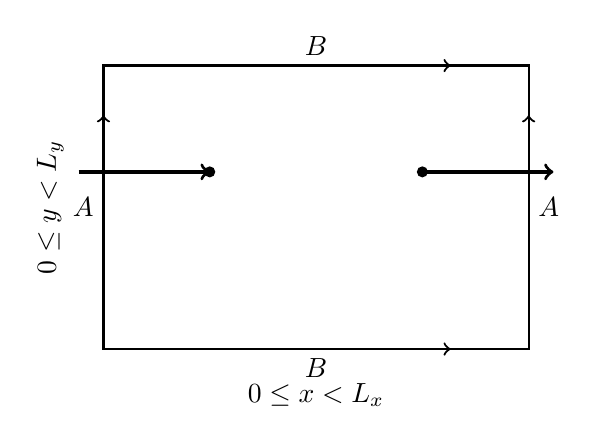
\begin{tikzpicture}[x=0.9cm,y=0.9cm]
\draw[thick] (0,0) rectangle (6,4);
\draw[->,thick] (0,0.7) -- (0,3.3);
\draw[->,thick] (6,0.7) -- (6,3.3);
\draw[->,thick] (1.1,0) -- (4.9,0);
\draw[->,thick] (1.1,4) -- (4.9,4);
\node[left] at (0,2) {$A$};
\node[right] at (6,2) {$A$};
\node[below] at (3,0) {$B$};
\node[above] at (3,4) {$B$};
\draw[->,very thick] (4.5,2.5) -- (6.35,2.5);
\draw[->,very thick] (-0.35,2.5) -- (1.5,2.5);
\fill (4.5,2.5) circle (2pt);
\fill (1.5,2.5) circle (2pt);
\node at (3,-0.65) {$0\leq x<L_x$};
\node[rotate=90] at (-0.75,2) {$0\leq y<L_y$};
\end{tikzpicture}
\caption{二次元の周期的空間：同じラベルをもつ辺は同一視されるので、一方の辺を横切った粒子は反対側の辺の対応する点に再び現れる。}
\end{figure}

\begin{classroomqa}
\lecturetimestamp{01:50:58}
\audiencequestion{周期的な構成は空間を表すのか、それとも空間内の対象を表すのか。}
\lecturerresponse{それは空間を表す。対象と場はその空間内に存在し、その同一視に従う。周期性は無限体積の問題を制御するために課され、体積を大きくして運動量の和を積分に置き換えることによって除去される。}
\end{classroomqa}

三次元の類似物は、三対の向かい合う面が同一視された立方体である。左面と右面は同じであり、上面と下面は同じであり、前面と背面は同じである。いずれかの面を横切った粒子は、同一視された相手の面を通って再び現れる。\footnote{周期的な立方体と、その三対の同一視された面は、01:51:27--01:52:17 に従う。\(k_i\) について表示された式は、先の条件 \(kL=2\pi n\) を三つの周期的な方向に適用して成分ごとに再構成したものである。} 三つの運動量成分は次を満たす。
\begin{equation}
k_i=\frac{2\pi n_i}{L_i},
\qquad i=x,y,z,
\end{equation}
各方向に対して一つの整数 \(n_i\) をもつ。トーラスは同じ規則によって任意の次元で定義できる。

\begin{figure}[t]
\centering
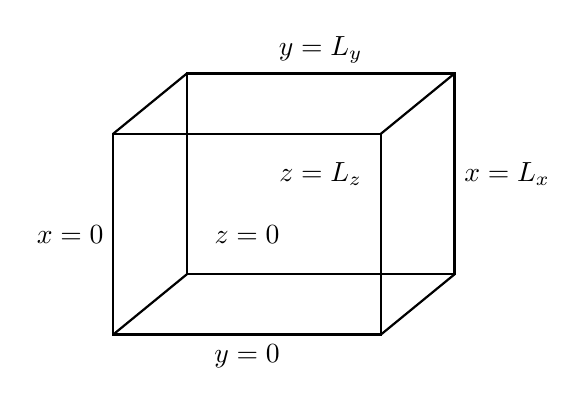
\begin{tikzpicture}[scale=0.85]
\draw[thick] (0,0) rectangle (4,3);
\draw[thick] (1.1,0.9) rectangle (5.1,3.9);
\draw[thick] (0,0) -- (1.1,0.9);
\draw[thick] (4,0) -- (5.1,0.9);
\draw[thick] (4,3) -- (5.1,3.9);
\draw[thick] (0,3) -- (1.1,3.9);
\node[left] at (0,1.5) {$x=0$};
\node[right] at (5.1,2.4) {$x=L_x$};
\node[below] at (2,0) {$y=0$};
\node[above] at (3.1,3.9) {$y=L_y$};
\node at (2,1.5) {$z=0$};
\node at (3.1,2.4) {$z=L_z$};
\end{tikzpicture}
\caption{三次元の周期的空間を、各対の向かい合う面が同一視された立方体として表したもの。}
\end{figure}

\begin{classroomqa}
\lecturetimestamp{01:52:20}
\audiencequestion{場の理論は空間に対して物理的な格子サイズを選ぶのか。}
\lecturerresponse{それは推測的な問いである。ここでの実用的な目的のためには、空間は連続である。量子は粒子であり、空間格子のセルではない。円の構成では、離散的になるのは運動量であり、位置は連続かつ周期的なままである。}
\end{classroomqa}

\editorialnote{格子サイズのやり取りの間に長く損傷した箇所があり、プランクスケールに言及しているが、空間の基本的な離散性について回復可能な主張を保持していない。ここではそのような主張は推論されない。}

\(k\) の離散性は、周期的な波動関数を課すことから完全に生じた。それは座標 \(x\) 自体が格子点上にある証拠ではない。空間が基本的な微視的構造をもつかもしれないと問うことは正当であるが、それは別個の推測的な問題である。

\section{フェルミオンと外部場}

ボソン的モードは任意の非負の占有数を許す。フェルミオンは反対の振る舞いを要求する。パウリの排他原理は、二つの同一のフェルミオンが同じ状態を占めることを禁じる。

\begin{classroomqa}
\lecturetimestamp{01:55:13}
\audiencequestion{交換子を反交換子に置き換えると、最も単純なフェルミオン理論が得られるのか。}
\lecturerresponse{本質的には、はい。交換子は \([A,B]=AB-BA\) であるのに対し、反交換子は \(\{A,B\}=AB+BA\) である。対応するフェルミオン的生成消滅代数はパウリの排他原理を実現する。すなわち、二番目の同一のフェルミオンをすでに占有された状態に入れることはできない。詳細な理論は後回しにする。}
\end{classroomqa}

二つの積は符号だけ異なる。
\begin{equation}
[A,B]=AB-BA,
\qquad
\{A,B\}=AB+BA.
\end{equation}
交換子は交換の下で反対称であるのに対し、反交換子は対称である。反交換子が消えるならば、
\begin{equation}
\{A,B\}=0
\quad\Longrightarrow\quad
AB=-BA.
\end{equation}
そのような対に対して、二つのフェルミオン演算子を交換すると符号が変わる。これは、\([A,B]=0\) から \(AB=BA\) が得られる通常の可換の場合よりも異常である。ボソン的交換子を対応する反交換代数に置き換えることが、フェルミオンに導く数学的変更である。その詳細な展開は延期する。

反交換関係は、ボソンで見られた統計的振る舞いを逆転させる。同一のフェルミオンが一つのモードに誘導的に積み重なることはない。そのモードの占有は、別の同一フェルミオンがそこへ入ることを妨げる。単一のフェルミオン状態は高々一つの同一フェルミオンしか含むことができないので、その一つの状態に任意に多数のフェルミオンを入れて得られる古典場の極限は存在しない。

\begin{classroomqa}
\lecturetimestamp{01:58:03}
\audiencequestion{フェルミオンからできているのに、なぜアルファ粒子はボソンになり得るのですか。}
\lecturerresponse{偶数個のフェルミオン的構成要素を含む束縛された複合体は、ボソン的統計を持ち得る。そのような複合ボソンをいくつか同一の全状態に入れることは、それらの個々のフェルミオン的構成要素を一つの同一な一粒子状態に入れることと同じではない。}
\end{classroomqa}

複合体の統計は、束縛された対象を全体として扱うものである。したがって、フェルミオン的構成要素は、構成要素に対する排他律に反することなく、ボソンとして振る舞う対象へと結合し得る。

\begin{classroomqa}
\lecturetimestamp{01:58:33}
\audiencequestion{外部場はどのように取り入れられるのですか。}
\lecturerresponse{これまでの構成には、外部の背景場は何も含まれていない。そのような場は古典場として指定することもできるし、多数の量子を含む状態によって量子力学的に表すこともできる。}
\end{classroomqa}

二つの記述が一致するには、大きな占有数の状態が適切に準備され、位相コヒーレントでなければならない。粒子数だけでは十分ではない。\footnote{交換関係が多量子スケールを与える。位相コヒーレンスは、大きな占有数だけでは古典場と誤認されないための追加条件としてここで述べられている。} その半古典的領域では、両者の効果は小さな量子的ずれを除いて一致する。これは基本的な整合性条件である。電磁場は、個々の量子が問題となる場合には離散的な光子を記述しなければならないが、多数の光子を含む適切に位相コヒーレントな状態は、古典電磁波のよく知られた作用を再現しなければならない。
